\clearpage
\section{CƠ SỞ LÝ THUYẾT VỀ LƯỚI ĐIỆN SIÊU NHỎ DC}
Chương này trình bày cơ sở lý thuyết về mạng điện, lưới điện siêu nhỏ và điều khiển lưới điện siêu nhỏ. Mục tiêu của chương là xây dựng một khung lý thuyết cho các nguyên lý được sử dụng trong phần còn lại của nghiên cứu này. \par
Trong mục 2.1 và 2.2, các lý thuyết và xu hướng của lưới điện siêu nhỏ DC được trình bày nhằm nhấn mạnh tầm quan trọng của việc điều khiển chúng — không chỉ ở hiện tại mà còn trong tương lai. Mục 2.3 nêu bật các chiến lược điều khiển khác nhau đang được đề cập trong các tài liệu hiện nay, đồng thời đi sâu vào một phương pháp điều khiển cụ thể mà các phần sau của nghiên cứu này sẽ tiếp tục phát triển. \par

\subsection{Các thành phần cấu tạo nên lưới điện siêu nhỏ DC}
\subsubsection{Các bộ biến đổi điện tử công suất}
Như đã đề cập, thành phần trung tâm của các hệ thống vi lưới (microgrids) nói chung — bất kể là vi lưới AC, DC hay lai AC-DC — chính là bộ biến đổi công suất, thiết bị kết nối giữa các nguồn năng lượng và tải tiêu thụ. Trong tiểu mục này, các mô hình động được thiết lập cho một số loại bộ biến đổi công suất thường được sử dụng trong vi lưới DC. \par
Theo [40], các cấu trúc bộ biến đổi DC có thể được phân thành hai nhóm: bộ biến đổi bậc hai (ví dụ: buck, boost, buck-boost, buck-boost không nghịch đảo) và bộ biến đổi bậc bốn (ví dụ: Cuk, Sepic, Zeta, buck bậc hai/quadratic buck). \par
Xét theo số lượng khóa chuyển mạch, các bộ biến đổi này cũng có thể được phân loại thành hai nhóm: đơn biến (mono-variable) hay còn gọi là đầu vào đơn đầu ra đơn (SISO - \textit{Single Input Single Output}), và đa biến (multi-variable) hay đầu vào/đầu ra đa kênh (MIMO - \textit{Multiple Input Multiple Output}). Ngoài ra, cũng tồn tại các bộ biến đổi có nhiều khóa chuyển mạch phụ thuộc lẫn nhau, và các bộ này cũng có thể được phân loại thành SISO hoặc MIMO. \par
\paragraph{Bộ biến đổi hạ áp (Buck Converter)}
Các bộ biến đổi Buck thuộc nhóm mạch cắt (chopper) hoặc mạch suy giảm (attenuation). Cụ thể, điện áp đầu ra được xác định bởi việc nhân điện áp đầu vào không đổi với một hệ số vô hướng, nhỏ hơn 1. Hình \ref{fig:C2_1} trình bày mạch điện của bộ biến đổi Buck bao gồm một phần tử chuyển mạch nối tiếp với nguồn và được điều khiển bởi đầu vào điều khiển $u$, nằm trong khoảng [0, 1], một đi-ốt song song $D$, một cuộn cảm $L$ nối tiếp và một tụ điện đầu ra $C$, cung cấp cho một tải tổng quát. \par
\begin{figure}
    \centering
    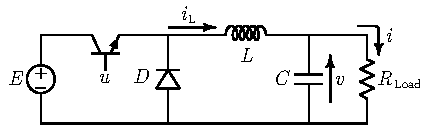
\includegraphics[width= 0.7 \textwidth]{Figures/Content_Pages/Chapter_2/C2_1.pdf}
    \caption{Mạch giảm áp (DC/DC Buck Converter)}
    \label{fig:C2_1}
\end{figure}
Bằng cách áp dụng các định luật Kirchhoff cho mạch điện trên, ta thu được mô hình trung bình được mô tả bởi các phương trình vi phân tuyến tính sau: \par
\begin{equation} \label{E2_1}
    L\frac{di_L}{dt} = -v+uE
\end{equation}
\begin{equation} \label{E2_2}
    C\frac{dv}{dt} = i_L - i 
\end{equation}
\noindent Trong đó, $i_L$, $E$, $i$ và $v$ lần lượt là dòng điện ngõ vào/ra và điện áp ngõ vào/ra của bộ biến đổi. \par
Việc sử dụng các bộ biến đổi giảm áp đã được ưu tiên rộng rãi trong nhiều ứng dụng lưới điện siêu nhỏ lý thuyết [22, 41–45], chủ yếu do động lực tuyến tính của chúng yêu cầu cấu trúc điều khiển đơn giản hơn. Kiến trúc một lưới điện DC được nghiên cứu trong [41], bao gồm một bộ biến đổi giảm áp cấp nguồn cho tải công suất hằng số (CPL), trong đó một bộ điều khiển hồi tiếp kết hợp với chiến lược điều khiển tiên đoán được đề xuất. Trong [43], các tác giả cố gắng giải quyết vấn đề mất ổn định của các bộ biến đổi giảm áp với CPL trong lưới điện DC bằng cách sử dụng một bộ điều khiển phi tuyến vững chắc. Một bộ điều khiển dự đoán mô hình (MPC) không sai lệch cho bộ biến đổi giảm áp với CPL nhằm đảm bảo hiệu năng mong muốn và đảm bảo ổn định được đề xuất trong [44]. Các tác giả trong [45] đánh giá hiệu suất chuyển đổi năng lượng của bộ biến đổi giảm áp ba mức khi hoạt động trong lưới điện DC hai cực không cân bằng. \par
Việc sử dụng các bộ biến đổi giảm áp đã được mở rộng trong nhiều ứng dụng của lưới điện siêu nhỏ DC, ví dụ như trên tàu thủy [46], các trang trại điện gió [47], trang trại điện mặt trời [48], hệ thống lưu trữ năng lượng [49] và các ứng dụng lưới điện siêu nhỏ DC điện áp thấp (LVDC MG) [50]. \par
Tuy nhiên, việc giả định rằng lưới điện siêu nhỏ DC chỉ bao gồm các bộ biến đổi Buck kết nối trực tiếp với nguồn năng lượng là điều không thực tế, bởi vì năng lượng được tạo ra từ nguồn thường có điện áp thấp và dòng điện cao, do đó thông thường cần được giao tiếp với phần còn lại của mạng thông qua một bộ biến đổi Boost. \par
\paragraph{Bộ biến đổi tăng áp (Boost Converter)}
Vì điện áp đầu ra của hầu hết các nguồn năng lượng phân tán như pin nhiên liệu và pin mặt trời (PV) thường khá thấp và hoạt động ở dòng điện cao, nên trong các ứng dụng thực tế, việc sử dụng bộ biến đổi tăng áp (\textit{step-up converter}) là cần thiết [51–55]. \par
\begin{figure}[!b]
    \centering
    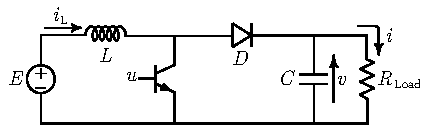
\includegraphics[width= 0.7 \textwidth]{Figures/Content_Pages/Chapter_2/C2_2.pdf}
    \caption{Mạch tăng áp (DC/DC Boost Converter)}
    \label{fig:C2_2}
\end{figure}
Thường được gọi là bộ biến đổi tăng áp trong các tài liệu chuyên ngành, cấu trúc mạch bộ biến đổi Boost được mô tả trong Hình \ref{fig:C2_2}. Cấu trúc của nó bao gồm một cuộn cảm đầu vào \( L \), kèm theo một phần tử chuyển mạch mắc song song được điều khiển bởi tín hiệu đầu vào \( u \), một diode mắc nối tiếp \( D \), và một tụ điện đầu ra \( C \), cung cấp điện cho một tải bất kỳ. \par
Áp dụng các định luật Kirchhoff, động lực học của bộ biến đổi Boost được mô tả bởi hệ phương trình vi phân sau: \par
\begin{equation} \label{E2_3}
    L\frac{di_L}{dt} = -(1-u)v +E
\end{equation}
\begin{equation} \label{E2_4}
    C \frac{dv}{dt} = (1-u)i_L - i
\end{equation}
\noindent Trong đó, $i_L$, $E$, $i$ và $v$ lần lượt là dòng điện ngõ vào/ra và điện áp ngõ vào/ra của bộ biến đổi. \par
\begin{figure}
    \centering
    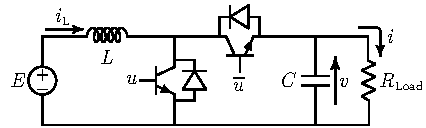
\includegraphics[width= 0.7 \textwidth]{Figures/Content_Pages/Chapter_2/C2_3.pdf}
    \caption{Mạch tăng áp hai chiều (Bidirectional DC/DC Boost Converter)}
    \label{fig:C2_3}
\end{figure}
Nhận xét 1: Với động lực học tương tự, ta có thể xây dựng bộ biến đổi boost hai chiều (Bidirectional Boost Converter) — hoạt động như một bộ tăng áp theo chiều thuận và hạ áp theo chiều ngược lại. Sự khác biệt duy nhất nằm ở chỗ diode \(D\) được thay thế bằng một phần tử chuyển mạch khác nhằm cho phép dòng công suất hai chiều. Mạch điện tử của bộ biến đổi boost hai chiều được minh họa trong Hình \ref{fig:C2_3}.\par
Trong [53], một bộ biến đổi boost liên tầng (\textit{interleaved boost converter}) với mạch nâng áp phụ kiểu Cuk có ghép từ được đề xuất nhằm đạt được hệ số nâng áp cần thiết bằng cách sạc một mạch nhân áp (\textit{voltage-doubler}) ở đầu ra. Một giải pháp tương tự được trình bày trong [54], trong đó một bộ biến đổi boost tích hợp sepic được giới thiệu, cung cấp khả năng nâng áp bổ sung thông qua một mạch nâng áp phụ kiểu sepic có cách ly. Tuy nhiên, các cấu trúc mạch của những bộ biến đổi nâng áp cao tích hợp Cuk/sepíc này tương đối phức tạp và tốn kém, do đó có thể khó sản xuất hàng loạt. Hơn nữa, trong thực tế, điện áp đầu ra tối đa và hiệu suất công suất có thể bị ảnh hưởng bởi các hiện tượng ký sinh, chẳng hạn như điện trở dây quấn của cuộn cảm trong các mạch tích hợp Cuk/sepíc. \par
Các bộ biến đổi boost đã được ứng dụng thành công trong các hệ thống điện mặt trời (PV) [61], pin nhiên liệu [62], pin sạc [63, 64] hoặc điện khí hóa nông thôn [65]. Tuy nhiên, do đặc tính phi tuyến của chúng, động học (\textit{dymanic}) của bộ biến đổi Boost thường bị bỏ qua trong phân tích lý thuyết hệ thống. Hầu hết các phương pháp tiếp cận sử dụng các mô hình đơn giản hóa hoặc mô hình bậc thấp, như trong [66, 67]; một số khác thì hoàn toàn bỏ qua động học của các bộ biến đổi và chỉ tập trung vào khung điều khiển và/hoặc tải được cấp nguồn [24, 68].\par
\paragraph{Bộ chỉnh lưu ba pha}
Tùy thuộc vào ứng dụng, như đã đề cập trước đó, các kỹ thuật điều khiển PWM đã được ưu tiên sử dụng để điều khiển các bộ chỉnh lưu ba pha nhằm tạo dạng sóng điện áp và/hoặc dòng điện đầu ra [69]. \par
\begin{figure}
    \centering
    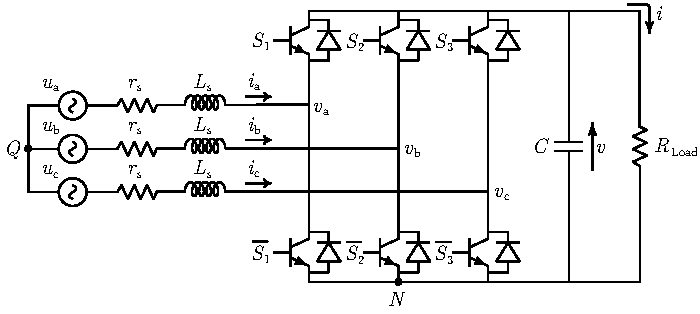
\includegraphics[width= \textwidth]{Figures/Content_Pages/Chapter_2/C2_4.pdf}
    \caption{Bộ chỉnh lưu AC/DC ba pha}
    \label{fig:C2_4}
\end{figure}
Sơ đồ của bộ chỉnh lưu AC/DC ba pha bao gồm ba nhánh với các transistor, như có thể thấy trong Hình \ref{fig:C2_4}, và còn được gọi là bộ chỉnh lưu boost hai chiều (bidirectional boost rectifier), hoạt động với cực tính điện áp DC cố định.\par
Áp dụng các định luật Kirchhoff, động lực học của bộ chỉnh lưu AC/DC ba pha được mô tả bởi hệ phương trình vi phân sau:
\begin{equation} \label{E2_5}
    L_s \frac{di_a}{dt} = -r_si_a - (v*S_1+V_{NQ}) + u_a
\end{equation}
\begin{equation} \label{E2_6}
    L_s \frac{di_b}{dt} = -r_si_b - (v*S_2+V_{NQ}) + u_b
\end{equation}
\begin{equation} \label{E2_7}
    L_s \frac{di_c}{dt} = -r_si_c - (v*3_2+V_{NQ}) + u_c
\end{equation}
\begin{equation} \label{E2_8}
    C \frac{dv}{dt} = (i_a *S_1) + (i_b*S_2) + (i_c *S_3) - i
\end{equation}
\noindent Các cuộn cảm \( L_s \) được lựa chọn dựa trên tiêu chí thiết kế nhằm bù hài. Các điện trở \( r_s \) đại diện cho điện trở ký sinh của cuộn cảm. Tụ điện \( C \) được sử dụng để đảm bảo dạng sóng điện áp được làm mượt. Các dòng điện \( i_a, i_b, i_c \) là dòng điện ba pha, trong khi \( u_a, u_b, u_c \) là các điện áp hình sin ba pha. Biến \( v \) là điện áp trên tụ điện, và \( V_{QN} \) là điện áp giữa hai điểm \( Q \) và \( N \). Các tín hiệu điều khiển \( S_j \), với \( j \in \{1, 2, 3\} \), được dùng để kích hoạt các khóa chuyển mạch, nhận giá trị trong khoảng đóng \([0, 1]\). \par
Theo như nghiên cứu [70], bằng cách sử dụng biến đổi Clarke và Park [71], mô hình toán học trong hệ tọa độ \(dq\) quay đồng bộ được thiết lập như sau:
\begin{equation} \label{E2_9}
    L \frac{dI_d}{dt} = -r_s I_d - \omega L_s I_q - m_d \frac{v}{2} + U_d
\end{equation}
\begin{equation} \label{E2_10}
    L \frac{dI_q}{dt} = -r_s I_q + \omega L_s I_d - m_q \frac{v}{2} + U_q
\end{equation}
\begin{equation} \label{E2_11}
    C \frac{dv}{dt} = \frac{3}{4} m_d I_d + \frac{3}{4} m_q I_q - i
\end{equation}
\noindent Trong đó, \(U_d\), \(U_1\) và \(I_d\), \(I_q\) lần lượt là điện áp và dòng điện ngõ vào trong hệ quy chiếu \(dq\). Đồng thời
\begin{equation} \label{E2_12}
    m_d = \frac{2v_d}{v}; \quad m_q = \frac{2v_q}{v}
\end{equation}
\noindent đại diện cho các đầu vào điều khiển theo tỷ lệ chu kỳ (duty-ratio). Các điện áp \( v_d \) và \( v_q \) là các thành phần \(d\) và \(q\) của điện áp chỉnh lưu \( [u_a\ u_b\ u_c]^T \). \par
Một bộ biến đổi AC/DC ba pha cách ly hai chiều sử dụng thuật toán điều chế vector không gian (SVPWM) cải tiến, giúp thực hiện chuyển đổi hai chiều AC/DC, tạo dòng xoay chiều hình sin và cách ly điện ở tần số cao đã được đề xuất trong [72]. Đối với một cấu hình được điều chỉnh nhẹ, bao gồm bộ biến đổi AC/DC ba pha có máy biến áp nối \( Y - \Delta \), một phương pháp điều khiển khác — nhưng vẫn đạt được kết quả cải thiện tương tự — được trình bày trong [73]. Nhiều ứng dụng lưới điện siêu nhỏ DC tích hợp các bộ chỉnh lưu ba pha trong cấu trúc của chúng. Ví dụ, một hệ thống chuyển đổi năng lượng gió (WECS) được trình bày trong [74], nơi một cầu chỉnh lưu diode ba pha kết hợp với bộ biến đổi DC/DC được kết nối tại đầu ra của máy phát không đồng bộ (induction generator) chạy bằng gió và lưới DC. Các lưới điện nhỏ (microgrid) sử dụng các bộ biến đổi AC/DC (hoặc DC/AC) ba pha cũng đã được nghiên cứu trong các tài liệu [75–79]. \par
Trong [80, 81], lưới điện siêu nhỏ DC tích hợp cả bộ chỉnh lưu ba pha hai chiều và các bộ biến đổi tăng áp Boost. Tuy nhiên, tương tự như các bộ biến đổi DC/DC tăng áp, mô hình động học phi tuyến của các bộ biến đổi ba pha trong lưới điện DC với điều khiển phi tuyến và tải phi tuyến, sau khi thực hiện biến đổi trong hệ tọa độ \(dq\), thường bị bỏ qua trong phân tích ổn định lý thuyết, trong khi sự chú trọng được đặt vào chiến lược điều khiển.
\subsubsection{Tải DC}
Trong các lưới điện DC, có nhiều loại tải khác nhau mà người ta có thể gặp. Gần đây, các tải theo mô hình ZIP trong các lưới điện siêu nhỏ DC ngày càng trở nên phổ biến hơn [82-88] \par
\begin{figure}
    \centering
    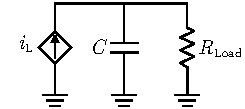
\includegraphics[width= 0.4\textwidth]{Figures/Content_Pages/Chapter_2/C2_5.pdf}
    \caption{Mạng điện một chiều đơn giản hóa với tải tổng quát}
    \label{fig:C2_5}
\end{figure}
\paragraph{Tải trở kháng không đổi (CIL)}

\paragraph{Tải dòng điện không đổi (CCL)}

\paragraph{Tải công suất không đổi (CPL)}

\subsection{Các cấu hình lưới điện siêu nhỏ DC}
Nhiều cấu trúc phần cứng của lưới điện vi mô DC đã được báo cáo, tùy thuộc vào từng ứng dụng cụ thể. Các tiêu chí cơ bản bao gồm tính linh hoạt trong điều khiển, độ bền vững và độ tin cậy. Các cấu trúc cơ bản của lưới điện vi mô DC có thể được phân loại thành ba nhóm chính \cite{dragivcevic2015dc}:\par
\subsubsection{Cấu hình thanh cái đơn}
Cấu trúc thanh cái đơn (single bus topology), được sử dụng phổ biến trong các lưới điện vi mô DC, đã được minh họa trong Hình 2.6 và tỏ ra hiệu quả trong các ứng dụng công nghiệp. Thanh cái DC trong cấu hình này bao gồm hai cực dương và âm. Một yếu tố quan trọng trong cấu trúc này là việc lựa chọn mức điện áp thanh cái DC, vì năng lượng được truyền dẫn qua một mức điện áp duy nhất [38]. \par
Khả năng truyền tải công suất được tăng cường nhờ mức điện áp cao hơn, tuy nhiên điều này cũng kéo theo việc tăng số lượng bộ chuyển đổi DC-DC trung gian nhằm đáp ứng yêu cầu về mức điện áp của thiết bị tiêu thụ [38]. Mức điện áp thấp sẽ giới hạn khả năng truyền tải công suất trong phạm vi khoảng cách ngắn. Tuy nhiên, cấu trúc này có thể rất hiệu quả ở các khu vực nông thôn xa xôi, nơi lưới điện quốc gia không khả thi. Một hệ thống thanh cái đơn 48V đã được triển khai cho các ngôi nhà ngoài lưới điện ở vùng nông thôn Ấn Độ [56]. \par
Cấu trúc điện áp thấp đã được đề cập rộng rãi trong nhiều tài liệu nghiên cứu [57,63] và có ưu điểm về tính đơn giản cũng như việc không phát sinh sự bất đối xứng giữa hai cực DC [38]. Tuy nhiên, một trong những nhược điểm của cấu trúc này là yêu cầu độ chính xác cao trong thiết kế mạch và các thông số điều khiển [37]. Ngoài ra, người sử dụng cũng không có tính dự phòng về mức điện áp cung cấp, vì họ chỉ được cấp điện thông qua một thanh cái duy nhất ở một mức điện áp cố định. \par
\subsubsection{Cấu hình nhiều thành cái}

\subsubsection{Các cấu hình khác}

\subsection{Các phương pháp điều khiển lưới điện siêu nhỏ DC}
\subsubsection{Phương pháp điều khiển tập trung}

\subsubsection{Phương pháp điều khiển phân phối}

\subsubsection{Phương pháp điều khiển phân phối}

\subsection{Sơ kết}